\documentclass[12pt, twoside]{article}
\usepackage[letterpaper, margin=1in, headsep=0.5in]{geometry}
\usepackage[english]{babel}
\usepackage[utf8]{inputenc}
\usepackage{amsmath}
\usepackage{amsfonts}
\usepackage{amssymb}
\usepackage{tikz}
\usepackage{yhmath}
\usetikzlibrary{quotes, angles}
\usepackage{graphicx}
\usepackage{enumitem}
\usepackage{multicol}

\newif\ifmeta
\metatrue %print standards and topics tags

\title{Regents Geometry}
\author{Chris Huson}
\date{April 2022}

\usepackage{fancyhdr}
\pagestyle{fancy}
\fancyhf{}
\renewcommand{\headrulewidth}{0pt} % disable the underline of the header
\raggedbottom

\fancyhead[LE]{\thepage}
\fancyhead[RO]{\thepage \\ Name: \hspace{4cm} \,\\}
\fancyhead[LO]{BECA / Dr. Huson / Geometry\\* Unit 11: Function transformations\\* 25 April 2022}

\begin{document}
\subsubsection*{11.1 Translation of a parabola \hfill HSG.CO.A.5}
\begin{enumerate}
\item Slide the rhombus $ABCD$ to the right six and up two. Label the image $A'B'C'D'$.
\begin{center}
    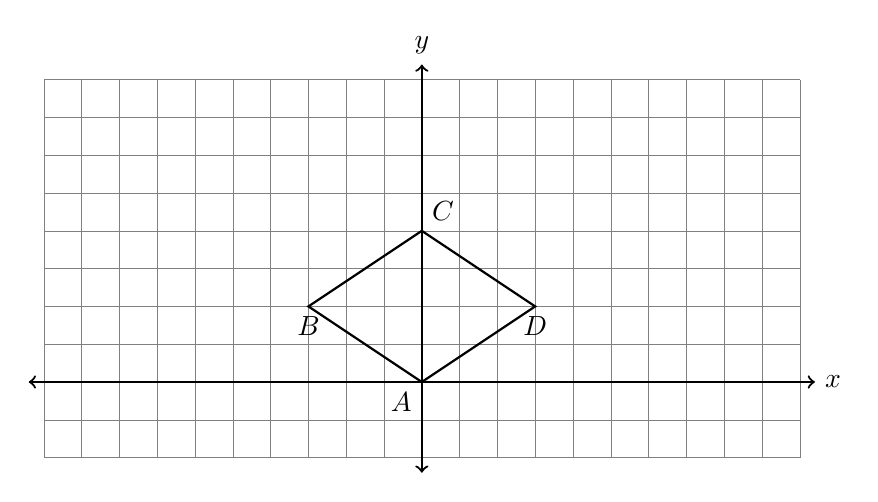
\begin{tikzpicture}[scale=.48]
    \draw [help lines] (-10,-2) grid (10,8);
    \draw [thick, <->] (-10.4,0) -- (10.4,0) node [right] {$x$};
    \draw [thick, <->] (0,-2.4)--(0,8.4) node [above] {$y$};  
    \draw [thick]
      (0,0) node[below left] {$A$}--
      (-3,2) node[below] {$B$}--
      (0,4) node[above right] {$C$}--
      (3,2) node[below] {$D$}--cycle;  
  \end{tikzpicture}
\end{center}

\item In the diagram below, $\overleftrightarrow{PQ}$ has the equation $\displaystyle y=-\frac{1}{2}x+3$.
\begin{multicols}{2}
  \begin{enumerate}
    \item Write down the slope of $\overleftrightarrow{PQ}$,\\[0.25cm] $m=$
    \item Write down the $y$-intercept of $\overleftrightarrow{PQ}$,\\[0.25cm] $b=$
    \item Translate the line up 2. Mark the images $P'$ and $Q'$.
    \item Write down the equation of $\overleftrightarrow{P'Q'}$
  \end{enumerate}
  \begin{flushright}
    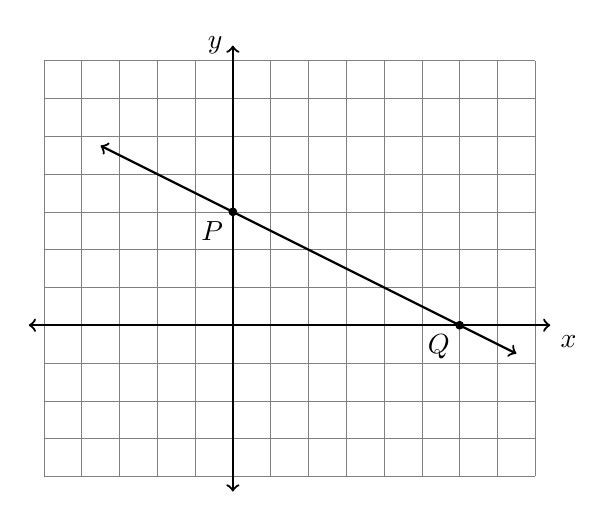
\begin{tikzpicture}[scale=.48]
      \draw [help lines] (-5,-4) grid (8,7);
      \draw [thick, <->] (-5.4,0) -- (8.4,0) node [below right] {$x$};
      \draw [thick, <->] (0,-4.4)--(0,7.4) node [left] {$y$};
      \draw [thick, <->] (-3.5,4.75)--(7.5,-0.75);
      \draw [fill] (0,3) circle [radius=0.1] node[below left] {$P$};
      \draw [fill] (6,0) circle [radius=0.1] node[below left] {$Q$};
    \end{tikzpicture}
  \end{flushright}
\end{multicols}\vspace{1cm}

\item Translate the parabola $f$ to the right three.
  \begin{center} 
  \begin{tikzpicture}[scale=0.8]
    \draw [thick, ->] (-5.2,0) -- (5.4,0) node [below right] {$x$};
    \draw [thick, ->] (0,-1.2)--(0,4.4) node [left] {$y$};
    \foreach \x in {-4,-3,-2,-1,1,2,3,4, 5} \draw (\x cm,3pt) -- (\x cm,-3pt) node[below] {$\x$};
    \draw [thick,<->,samples=20,domain=-2.7:2.7] plot(\x,\x*\x/2);
    \fill (0,0) circle[radius=0.1];
    \node at (-3,3){$f$};
  \end{tikzpicture}
  \end{center}
  
\newpage
\item Complete the t-table for the function $f$: $y=x^2$, plot the points, and draw $f$ as a smooth curve.
  \begin{center} 
  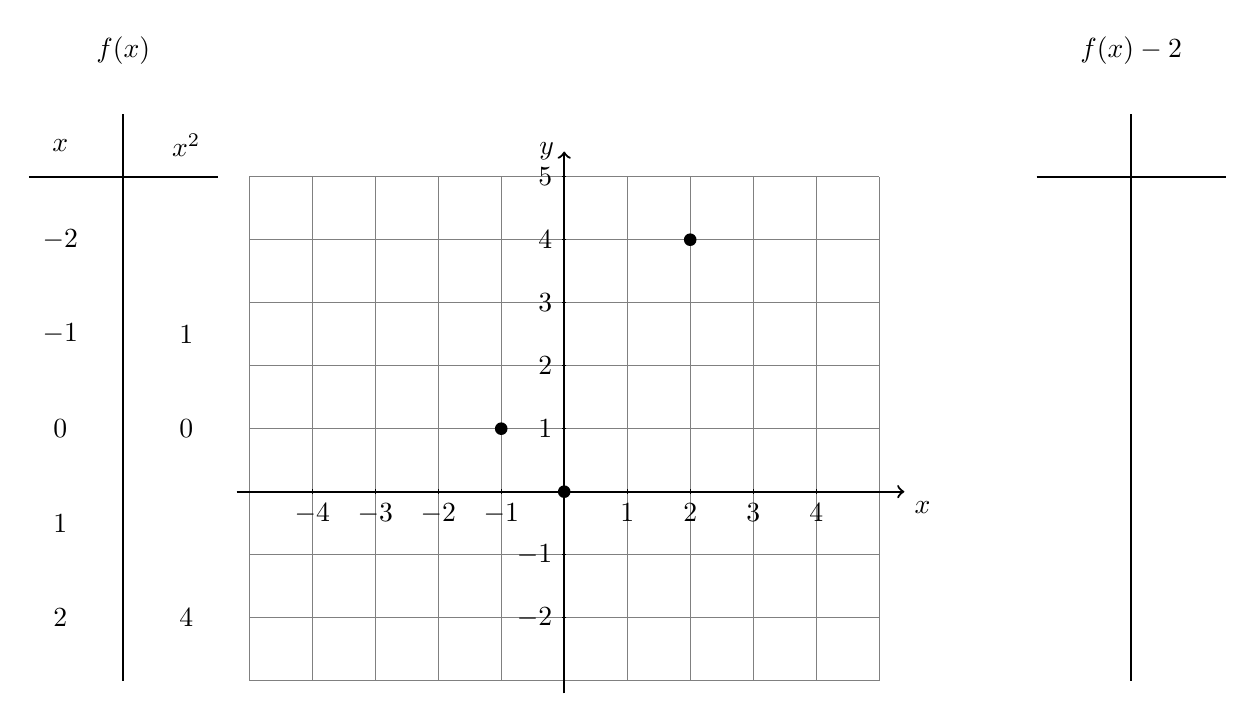
\begin{tikzpicture}[scale=0.8]
    \draw [help lines] (-5,-3) grid (5,5);
    \draw [thick, ->] (-5.2,0) -- (5.4,0) node [below right] {$x$};
    \draw [thick, ->] (0,-3.2)--(0,5.4) node [left] {$y$};
    \foreach \x in {-4,-3,-2,-1,1,2,3,4} \draw (\x cm,1pt) -- (\x cm,-1pt) node[below] {$\x$};
    \foreach \y in {-2,-1,1,2,3,4,5} \draw (1pt,\y cm) -- (-1pt,\y cm) node[anchor=east] {$\y$};

    %\draw [thick, <->,smooth,samples=20,domain=-2.3:2.35] plot(\x,\x*\x);

    \draw [thick] (-7,-3) -- (-7,6);
    \draw [thick] (-8.5,5) -- (-5.5,5);
    \node at (-7,7){$f(x)$};
    \draw [thick] (9,-3) -- (9,6);
    \draw [thick] (7.5,5) -- (10.5,5);
    \node at (9,7){$f(x)-2$};
    \node at (-8,5.5){$x$}; \node at (-6,5.5){$x^2$};
    \node at (-8,4){$-2$};
    \node at (-8,2.5){$-1$}; \node at (-6,2.5){$1$};
    \node at (-8,1){$0$};  \node at (-6,1){$0$};
    \node at (-8,-0.5){$1$};
    \node at (-8,-2){$2$}; \node at (-6,-2){$4$};
    %\fill (-2,4) circle[radius=0.1];
    \fill (-1,1) circle[radius=0.1];
    \fill (0,0) circle[radius=0.1];
    %\fill (1,1) circle[radius=0.1];
    \fill (2,4) circle[radius=0.1];
  \end{tikzpicture}
  \end{center}
  Translate the parabola $f$ down two and complete the t-table at right.
\vspace{1cm}

\item Two parabolas are shown below, $g(x)$ (solid line) and the parent function $y=x^2$ (dashed). What translation would map $g$ onto the parent?
\begin{center} 
\begin{tikzpicture}[xscale=1.0, yscale=1]
  \draw [thick, ->] (-5.2,0) -- (5.4,0) node [below right] {$x$};
  \draw [thick, ->] (0,-0.5)--(0,4.4) node [left] {$y$};
  \foreach \x in {-4,-3,-2,-1,1,2,3,4, 5} \draw (\x cm,3pt) -- (\x cm,-3pt) node[below] {$\x$};
  \foreach \y in {1,2,3,4} \draw (1pt,\y cm) -- (-1pt,\y cm) node[left] {$\y$};
  \draw [dashed,<->,samples=20,domain=-1.75:1.75] plot(\x,\x*\x);
  \fill (0,0) circle[radius=0.1];
  \draw [thick,<->,samples=20,domain=2.25:5.75] plot(\x,{(\x-4)^2+2});
  \fill (4,2) circle[radius=0.1];
  \node at (4.5,1.5){$(4,2)$};
  \node at (5,4.5){$g(x)$};
\end{tikzpicture}
\end{center}

\end{enumerate}
\end{document}
  